\documentclass[12pt]{article}
\usepackage[a4paper, margin=1in]{geometry} 
\usepackage{graphicx} 
\usepackage{hyperref}
\usepackage{float}
\usepackage{multicol}
\usepackage{multirow}
\usepackage{amsmath}
\usepackage[ruled]{algorithm2e}
\usepackage{amssymb}
\usepackage[font=small, labelfont=bf]{caption}
\usepackage[table,xcdraw]{xcolor}

\title{Lecture Notes for \\ INF281 Basics of Bioinformatics Sequence Analysis}
\author{Takaya Saito}
\date{}

\begin{document}

\pagenumbering{arabic}
\setcounter{page}{46}

\makeatletter 
\renewcommand{\thefigure}{\arabic{section}.\arabic{figure}}
\renewcommand{\thetable}{\arabic{section}.\arabic{table}}
\makeatother

%
% Evaluation of alignment scores
%
\setcounter{section}{5}
\setcounter{figure}{0}
\setcounter{table}{0}
\section{Evaluation of alignment scores}
%\documentclass[12pt]{article}
%\usepackage[a4paper, margin=1in]{geometry} 
%\usepackage{graphicx} 
%\usepackage{hyperref}
%\usepackage{float}
%\usepackage{multicol}
%\usepackage{multirow}
%\usepackage[font=small, labelfont=bf]{caption}
%
%\begin{document}

%
% Statistical analysis
%
\subsection{Statistical analysis}
Statistical tests are performed to give an explanation to observed alignment scores.

%
% Hypothesis testing
%
\subsubsection*{Hypothesis testing} 
\begin{itemize}
\item Alternative hypothesis
\item Null hypothesis
\end{itemize}

\begin{figure}[H]
  \centering
      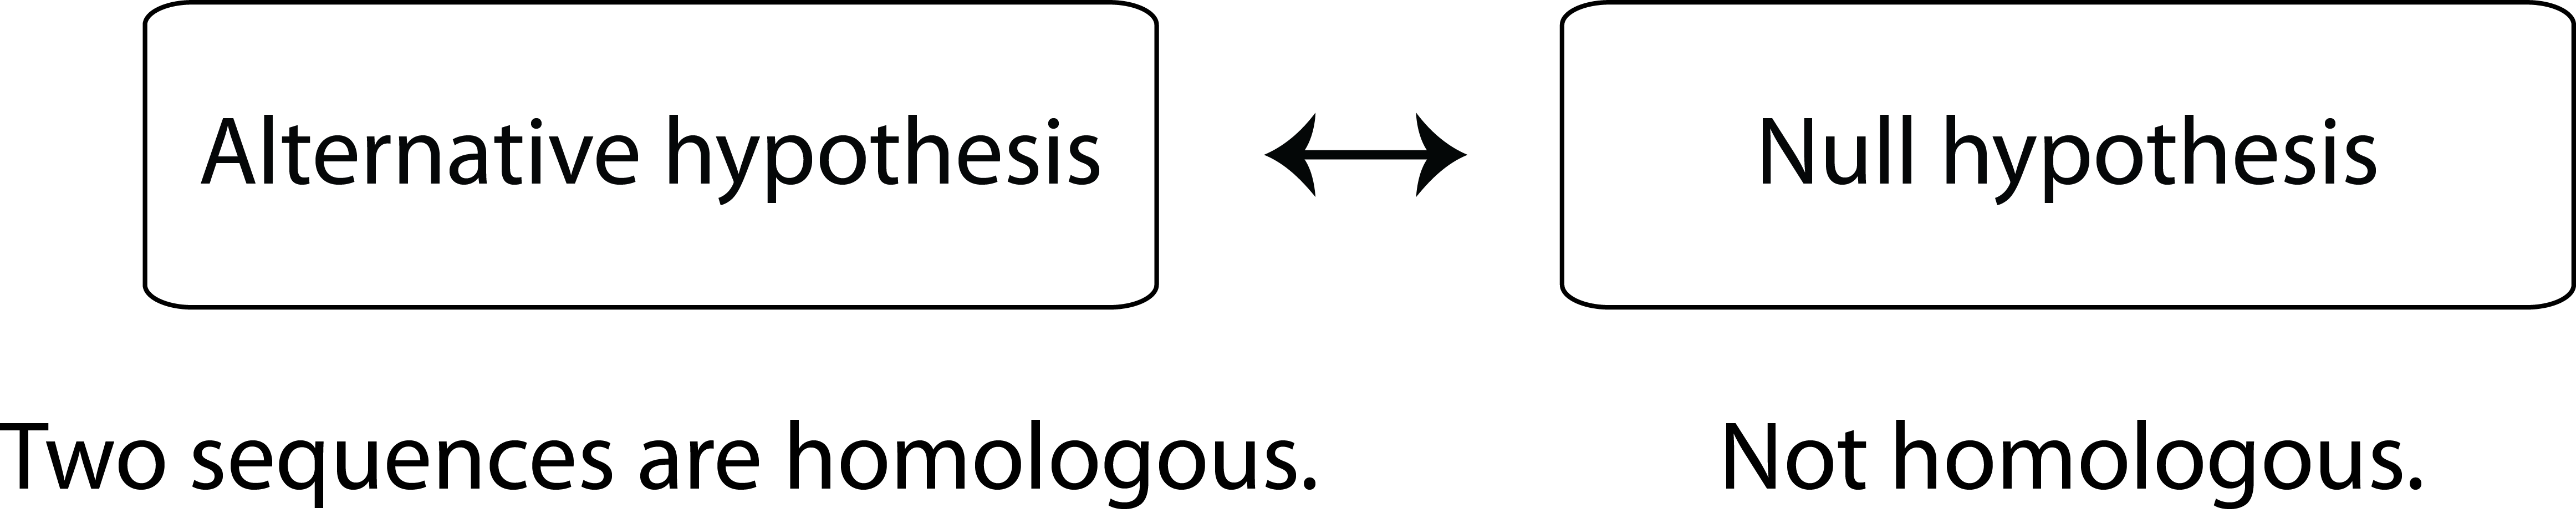
\includegraphics[width=0.6 \textwidth]{fig06/hypotheses.png}
  \caption{The null hypothesis and the alternative hypothesis}
\end{figure}

%
% P-value
%
\subsubsection*{P-value} 
``The p-value is defined as the probability of obtaining a result equal to or more extreme than what was actually observed, assuming that the null hypothesis is true'' \\

\noindent
-- the p-value page on Wikipedia (\url{https://en.wikipedia.org/wiki/P-value})

%
% Significance level (\alpha)
%
\subsubsection*{Significance level ($\alpha$)} 
The significance level should be chosen to indicate strong/weak evidence against the null hypothesis. \\

\noindent
Significance levels 0.05 and 0.01 are often used in life sciences.
\begin{itemize}
\item Statistically significant: $\alpha$ = 0.05
\item Statistically highly significant: $\alpha$ = 0.01
\end{itemize}

%
% Common misunderstandings of p-value
%
\subsubsection*{Common misunderstandings of p-value} 
``The p-value is not the probability that the null hypothesis is true or the probability that the alternative hypothesis is false.'' \\

\noindent
-- the p-value page on Wikipedia (\url{https://en.wikipedia.org/wiki/P-value})

%
% Underlying (background) score distributions
%
\subsubsection*{Underlying (background) score distributions} 
\begin{table}[H]
\centering
\caption{Alignment methods and distributions}
\begin{tabular}{ll}
Method                     & Underlying distribution \\ \hline
Global alignment           & Unknown                 \\
Local alignment (ungapped) & Gumbel                 
\end{tabular}
\end{table}

\bigskip 

%\end{document}

%\documentclass[12pt]{article}
%\usepackage[a4paper, margin=1in]{geometry} 
%\usepackage{graphicx} 
%\usepackage{hyperref}
%\usepackage{float}
%\usepackage{multicol}
%\usepackage{multirow}
%\usepackage[font=small, labelfont=bf]{caption}
%
%\begin{document}

%
% Evaluation of global alignment
%
\subsection{Evaluation of global alignment}
The underlying distribution of global alignment scores is unknown.

%
% Random generation of sequences
%
\subsubsection*{Random generation of sequences} 
One needs to consider using the appropriate length and compositions of amino acids or nucleotides needs when creating randomised sequences. \\

\noindent
\textbf{Example}

\noindent
Input sequences
\begin{verbatim}
    q: ACGT
    d: AGTACC  
\end{verbatim}

\noindent
Frequencies: {$f_{A}$ = 0.2, $f_{C}$ = 0.4, $f_{G}$ = 0.1, $f_{T}$ = 0.3} \\
Length: 6

\begin{verbatim}
    d1: CCAGTC
    d2: TCACCG
    d3: CTTGAA
    ...
\end{verbatim}

%
% Frequency distributions
%
\subsubsection*{Frequency distributions} 
\begin{itemize}
\item Universal (e.g. the whole protein database)
\item Global (e.g. protein super families)
\item Local (e.g. query and database sequences)
\end{itemize}

%
% Additional constrains
%
\subsubsection*{Additional constrains} 
Constrains on sequences generation are often considered. 
\begin{itemize}
\item Di-amino acid frequencies
\item Sub-region specific frequencies
\end{itemize}

%
% Non-parametric test and p-value
%
\subsubsection*{Non-parametric test and p-value} 
The simplest non-parametric test is calculating the rank of the score for the original alignment as the p-value. \\

$p=(b+1)/(n+1)$ \\

\noindent
where $b$ is the number of randomly generated scores above the score of the original alignment, and $n$ is the sample size. \\ 

\noindent
\textbf{N.B.} $n$ should be sufficiently large (e.g. $>$1000) to estimate an accurate p-value. \\

% NEWPAGE
\newpage

\noindent
\textbf{Example}

\begin{figure}[H]
  \centering
      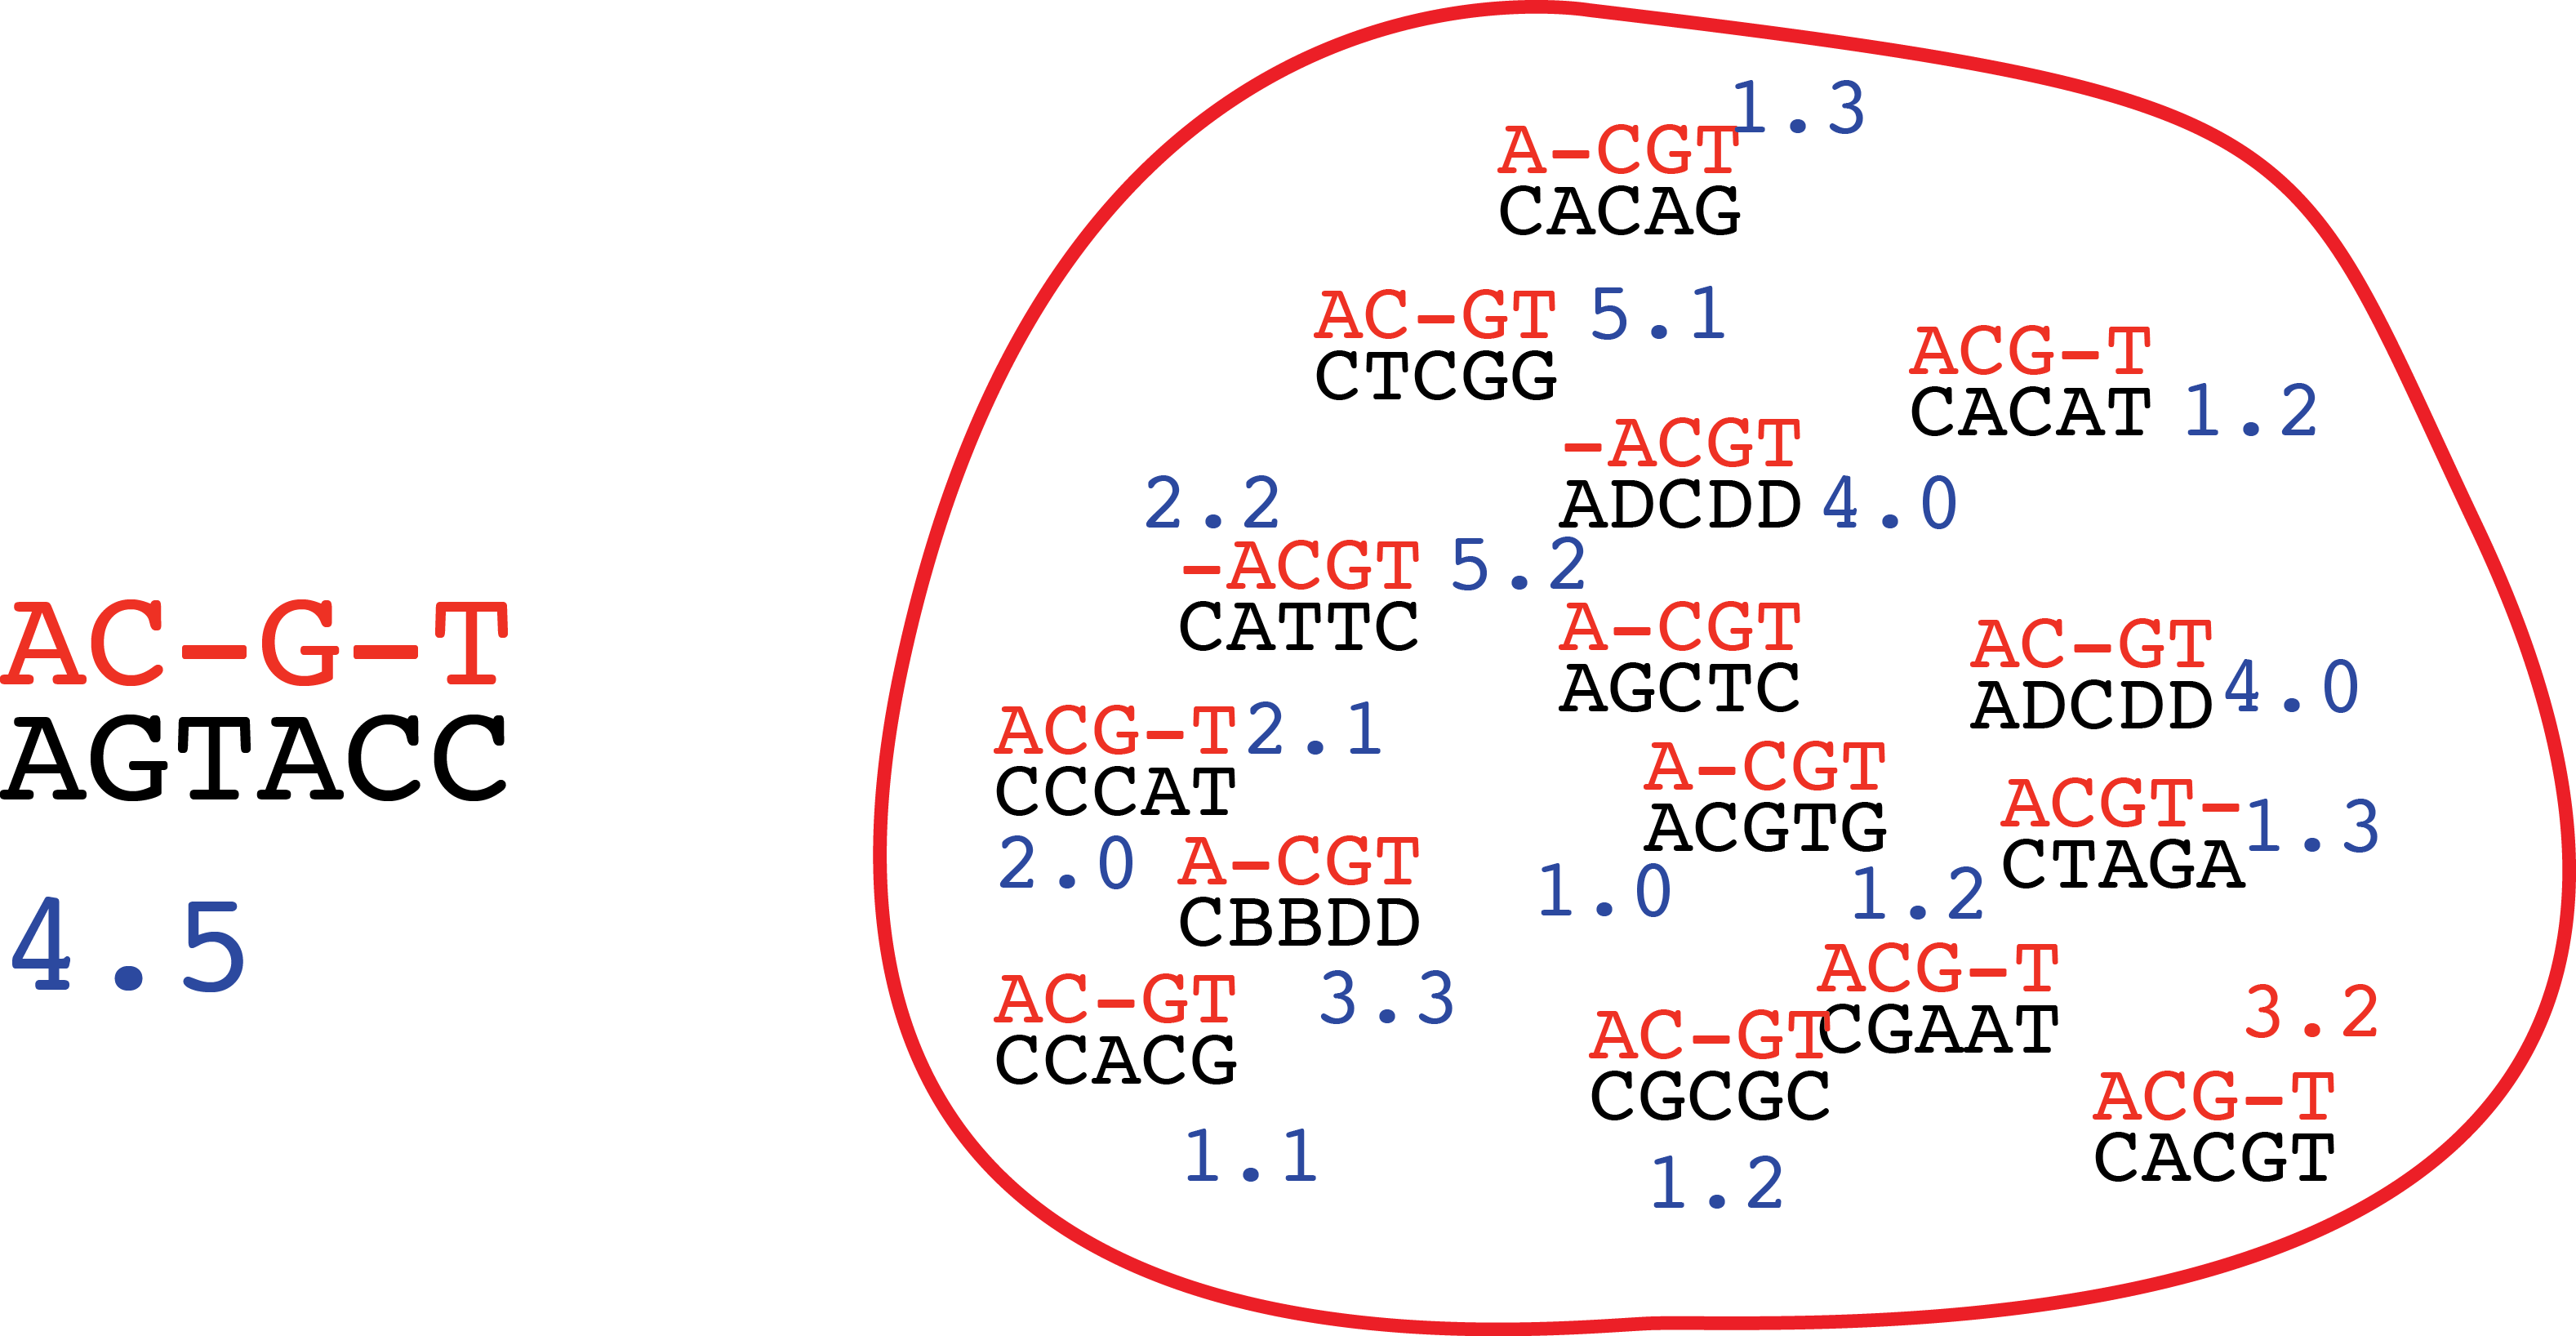
\includegraphics[width=0.5 \textwidth]{fig06/random_sequences.png}
  \caption{Randomly generated sequences and alignment scores}
\end{figure}

\begin{table}[H]
\centering
\tiny
\begin{tabular}{llllllllllllllllllll}
\hline
\multicolumn{1}{|l|}{1} & \multicolumn{1}{l|}{2}   & \multicolumn{1}{l|}{3}   & \multicolumn{1}{l|}{4}   & \multicolumn{1}{l|}{5}   & \multicolumn{1}{l|}{6}   & \multicolumn{1}{l|}{7}   & \multicolumn{1}{l|}{8}   & \multicolumn{1}{l|}{9}   & \multicolumn{1}{l|}{10}  & \multicolumn{1}{l|}{11}  & \multicolumn{1}{l|}{12} & \multicolumn{1}{l|}{13}  & \multicolumn{1}{l|}{14}  & \multicolumn{1}{l|}{15}  & \multicolumn{1}{l|}{16}  & \multicolumn{1}{l|}{17}  & \multicolumn{1}{l|}{18}  & \multicolumn{1}{l|}{19}  & \multicolumn{1}{l|}{20}  \\ \hline
\multicolumn{1}{|l|}{1} & \multicolumn{1}{l|}{1.1} & \multicolumn{1}{l|}{1.3} & \multicolumn{1}{l|}{1.4} & \multicolumn{1}{l|}{1.7} & \multicolumn{1}{l|}{2.1} & \multicolumn{1}{l|}{2.2} & \multicolumn{1}{l|}{2.2} & \multicolumn{1}{l|}{2.3} & \multicolumn{1}{l|}{2.5} & \multicolumn{1}{l|}{2.8} & \multicolumn{1}{l|}{3}  & \multicolumn{1}{l|}{3.2} & \multicolumn{1}{l|}{3.3} & \multicolumn{1}{l|}{3.4} & \multicolumn{1}{l|}{3.6} & \multicolumn{1}{l|}{4.2} & \multicolumn{1}{l|}{4.4} & \multicolumn{1}{l|}{4.7} & \multicolumn{1}{l|}{5.2} \\ \hline
                        &                          &                          &                          &                          &                          &                          &                          &                          &                          &                          &                         &                          &                          &                          &                          &                          & \multicolumn{2}{c}{\textbf{4.5}}                             &                         
\end{tabular}
\end{table}

p-value: $(2 + 1) / (20 + 1) = 0.1429$

\begin{itemize}
\item Significance level $\alpha = 0.2$:  reject the null hypothesis
\item Significance level $\alpha = 0.05$: the null hypothesis is not rejected
\end{itemize}

%
% Exercise \thesection.1
%
\subsubsection*{Exercise \thesection.1}

\begin{enumerate}
\item Calculate the frequencies of nucleotides from the four sequences below.

\begin{verbatim}
    d1: CCAGC
    d2: TCACG
    d3: CTTAA
    d4: AACAA
\end{verbatim}

Frequencies: \{$f_{A} = \quad$, $f_{C} = \quad$, $f_{G} =  \quad$, $f_{T} =  \quad$ \}

\item Calculate the p-value of the alignment below. 

\begin{verbatim}
    q: AACG
    d: A-CG
    Score: 40
\end{verbatim}

\noindent
Assume that the scores are pre-calculated for the alignments of the query sequence and nine randomly generated sequences as follows. Use them for the p-value calculation.

\begin{table}[H]
\centering
\small
\begin{tabular}{|l|l|l|l|l|l|l|l|l|l|}
\hline
\textbf{No.}   & 1 & 2  & 3  & 4  & 5  & 6  & 7  & 8  & 9  \\ \hline
\textbf{Score} & 4 & 14 & 33 & 45 & 74 & 76 & 82 & 83 & 94 \\ \hline
\end{tabular}
\end{table}


\end{enumerate}

\bigskip 

%\end{document}

%\documentclass[12pt]{article}
%\usepackage[a4paper, margin=1in]{geometry} 
%\usepackage{graphicx} 
%\usepackage{hyperref}
%\usepackage{float}
%\usepackage{multicol}
%\usepackage{multirow}
%\usepackage[font=small, labelfont=bf]{caption}
%\usepackage[table,xcdraw]{xcolor}
%
%\begin{document}

%
% Evaluation of local alignment
%
\subsection{Evaluation of local alignment}
The underlying distribution of local alignment scores is an extreme value distribution.

%
% Gumbel distribution
%
\subsubsection*{Gumbel distribution} 
The Gumbel distribution is a member of the extreme value distribution family. \\

\begin{figure}[H]
  \centering
      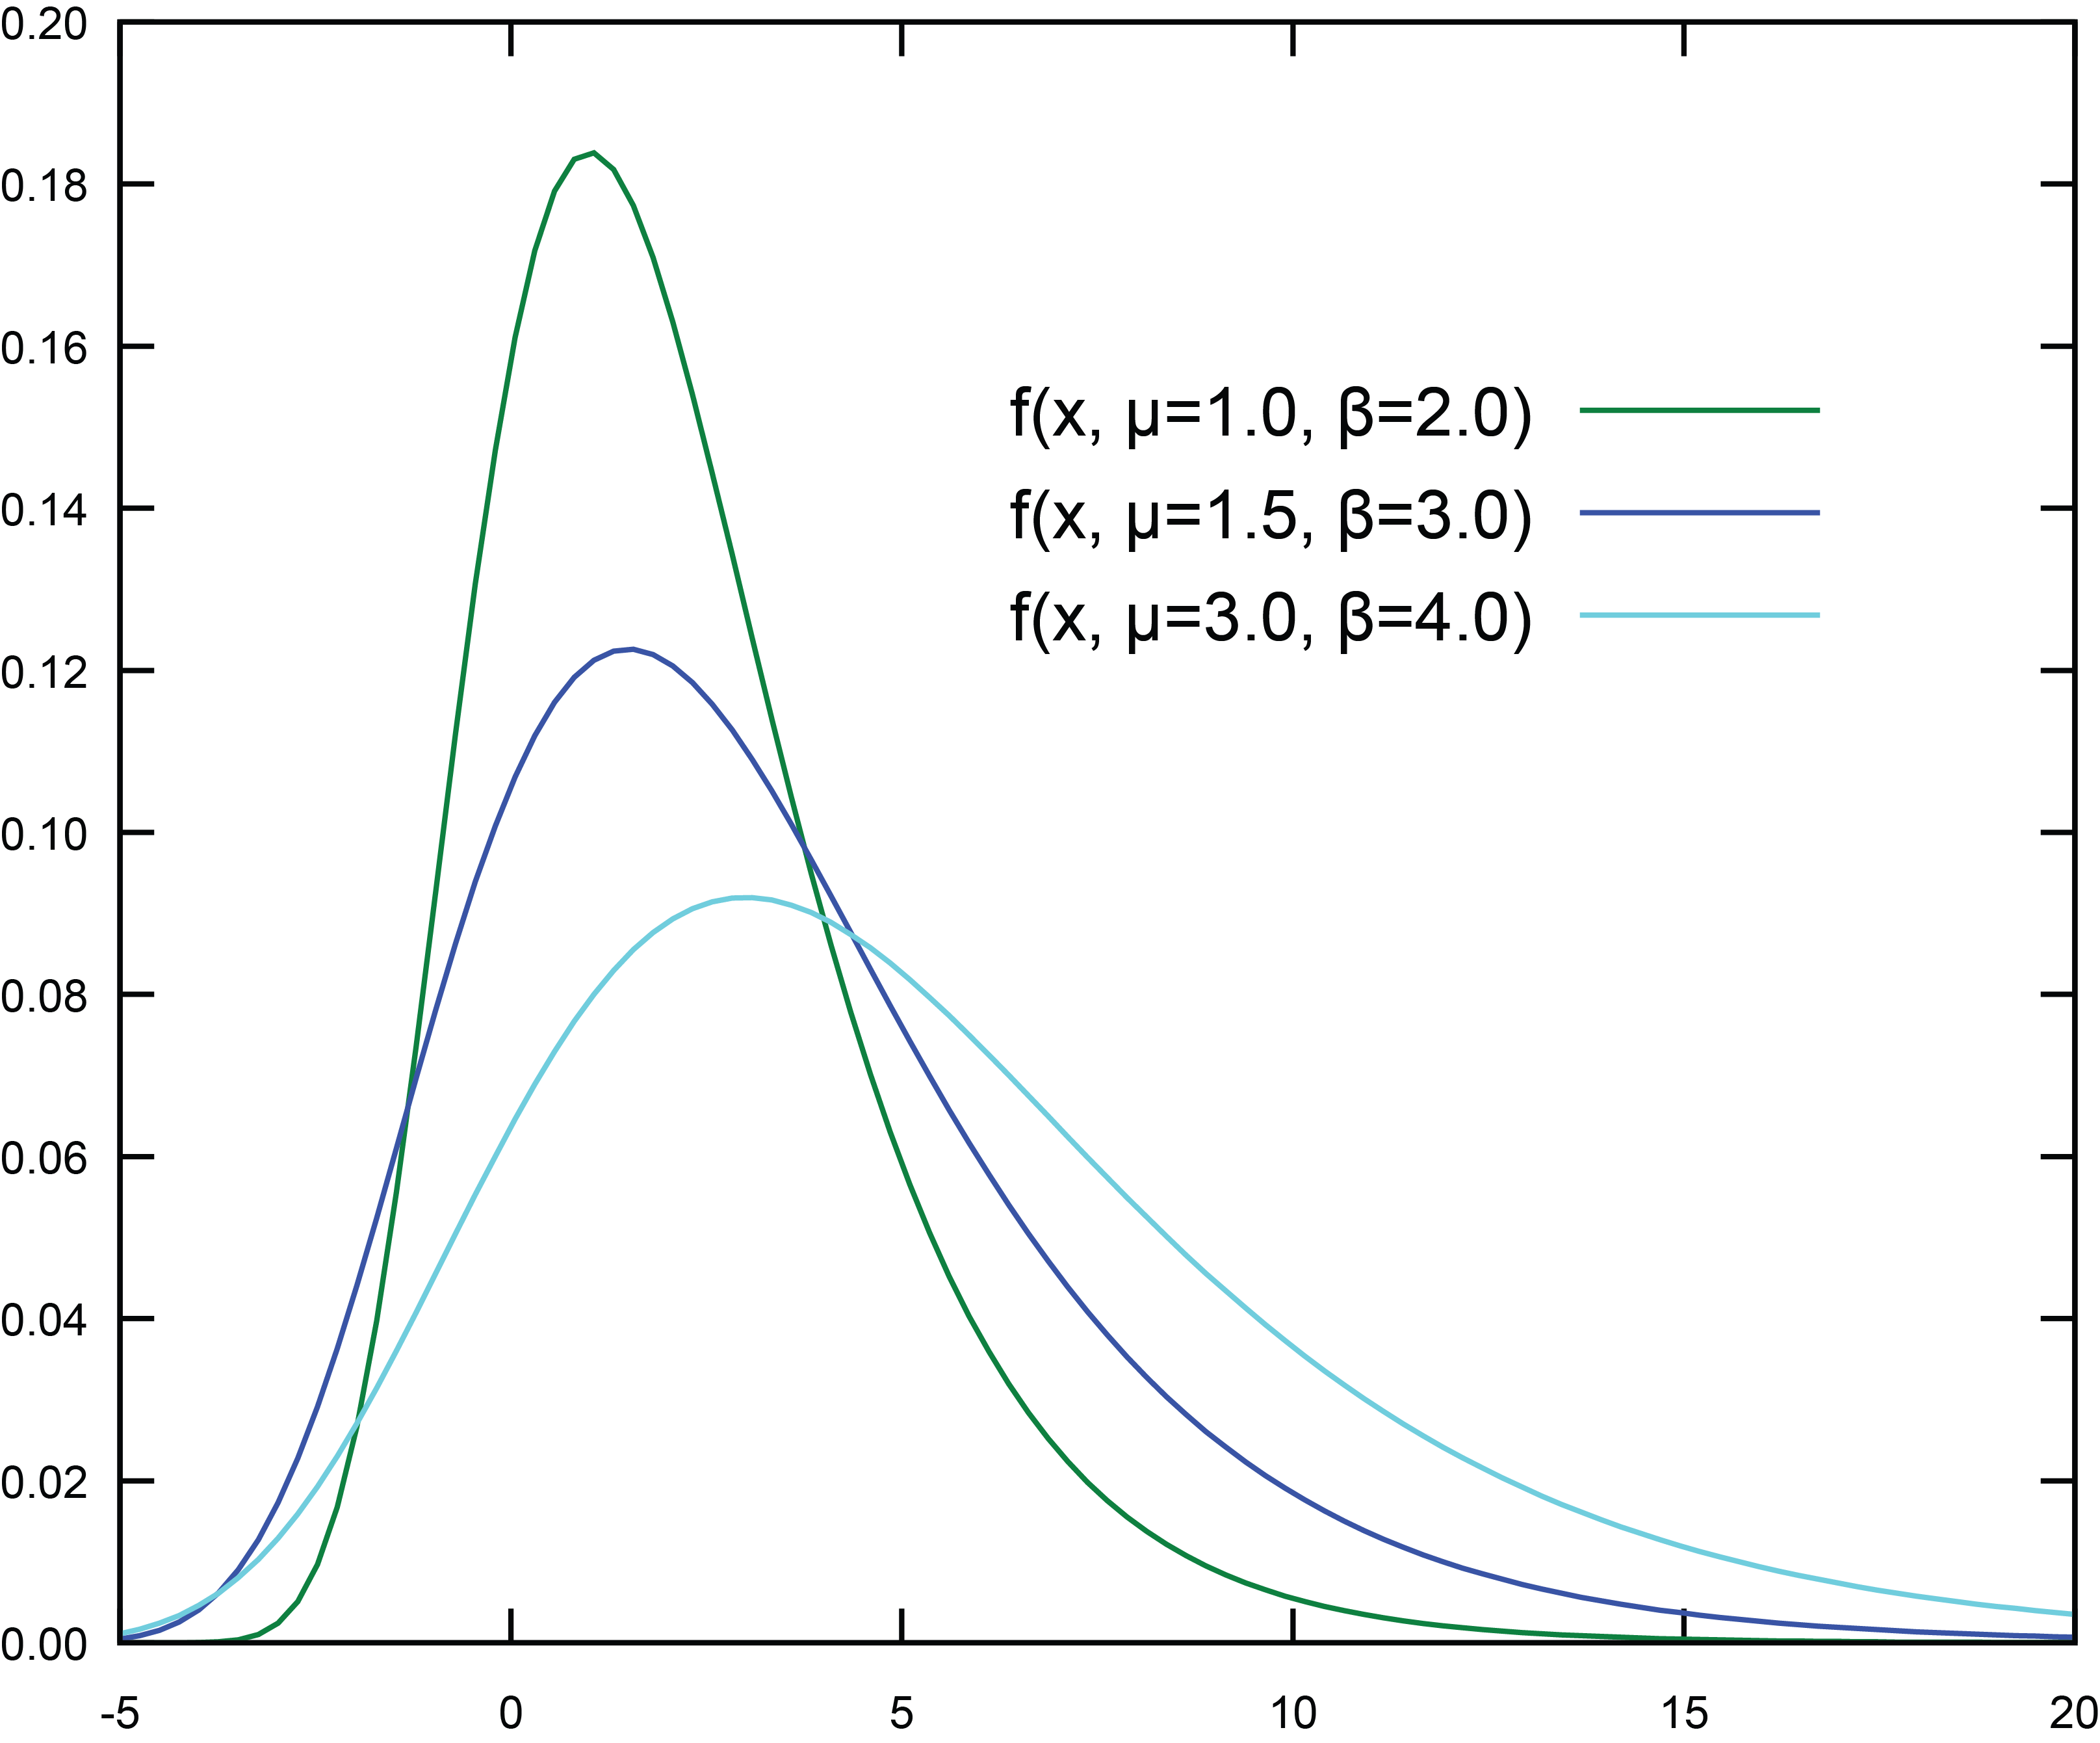
\includegraphics[width=0.4 \textwidth]{fig06/gumbel.png}
  \caption{Gumbel distribution (source: \href{https://commons.wikimedia.org/w/index.php?curid=4787663}{Herr blaschke, Wikimedia Commons})}
\end{figure}

\noindent
The cumulative distribution function (CDF) of the Gumbel distribution: \\
$F_Y(y) = exp⁡[-e^{-\lambda(y-\mu)}]$ \\

\noindent
Parameters
\begin{itemize}
\item $\mu$: the modal value of the distribution, characteristic value
\item $\lambda$: a measure of the variance, decay constant
\end{itemize}

%
% Extreme value distribution
%
\subsubsection*{Extreme value distribution}
An extreme value distribution is a limiting distribution for the minimum or the maximum of a sufficiently large sample. Ungapped alignments with large sequence lengths are known to have this type of distribution. \\

\noindent
\textbf{Example (m and n are not large in this example)}

\begin{table}[H]
\centering
\begin{tabular}{lllllllll}
                       &                        & A                        & C                                                & G                                              & C                        & A                        & C                                                & G                                              \\ \cline{2-9} 
\multicolumn{1}{l|}{}  & \multicolumn{1}{l|}{0} & \multicolumn{1}{l|}{0}   & \multicolumn{1}{l|}{0}                           & \multicolumn{1}{l|}{0}                         & \multicolumn{1}{l|}{0}   & \multicolumn{1}{l|}{0}   & \multicolumn{1}{l|}{0}                           & \multicolumn{1}{l|}{0}                         \\ \cline{2-9} 
\multicolumn{1}{l|}{C} & \multicolumn{1}{l|}{0} & \multicolumn{1}{l|}{0}   & \multicolumn{1}{l|}{\cellcolor[HTML]{FE0000}0.5} & \multicolumn{1}{l|}{0}                         & \multicolumn{1}{l|}{0.5} & \multicolumn{1}{l|}{0}   & \multicolumn{1}{l|}{\cellcolor[HTML]{FE0000}0.5} & \multicolumn{1}{l|}{0}                         \\ \cline{2-9} 
\multicolumn{1}{l|}{G} & \multicolumn{1}{l|}{0} & \multicolumn{1}{l|}{0}   & \multicolumn{1}{l|}{0}                           & \multicolumn{1}{l|}{\cellcolor[HTML]{FE0000}1} & \multicolumn{1}{l|}{0.5} & \multicolumn{1}{l|}{0.2} & \multicolumn{1}{l|}{0}                           & \multicolumn{1}{l|}{\cellcolor[HTML]{FE0000}1} \\ \cline{2-9} 
\multicolumn{1}{l|}{A} & \multicolumn{1}{l|}{0} & \multicolumn{1}{l|}{0.5} & \multicolumn{1}{l|}{0}                           & \multicolumn{1}{l|}{0.5}                       & \multicolumn{1}{l|}{0.7} & \multicolumn{1}{l|}{0.2} & \multicolumn{1}{l|}{0}                           & \multicolumn{1}{l|}{0.5}                       \\ \cline{2-9} 
\end{tabular}
\end{table}

\begin{table}[H]
\centering
\begin{tabular}{
>{\columncolor[HTML]{FE0000}}l |
>{\columncolor[HTML]{FE0000}}l |l|l|l|l|l}
CG & CG & GC  &     & AC   &     &     \\
CG & CG & GA  & ... & CG   & ... & ... \\ \hline
1  & 1  & 0.2 &     & -0.6 &     &    
\end{tabular}
\end{table}

%
% Parameter estimation
%
\subsubsection*{Parameter estimation}
The p-value of the Gumbel distribution can be calculated as: \\

$P[Y>y]=1-F_Y (y)=1-exp⁡[-e^{-\lambda(y-\mu)}]$ \\

\noindent
The parameters $\mu$ and $\lambda$ can be estimated from the arithmetic mean $m_{Y}$ and the variance $\sigma_{Y}^2$ of the observed sample. \\

$\lambda \approx 1.282 / \sigma_{Y}$ \\

$\mu \approx m_{Y} - 0.577/\lambda$

%
% Example of parameter estimation
%
\subsubsection*{Example of parameter estimation}
Below is the optimal local alignment with the score between q:ACAGACTACTA and  d:TCAGACTGGGAACCE.

\begin{verbatim}
    CAGACT
    CAGACT
    Score: 6
\end{verbatim}

\noindent
The mean and the variance of the alignment scores are estimated as follows from randomly generated sequences. \\

$m_{Y}$: 1.7221 \\

$\sigma_{Y}$: 1.6025 \\

\noindent
Then, $\lambda$ and $\mu$ are estimated from $m_{Y}$ and $\sigma_{Y}$. \\

$\lambda \approx 1.282 / 1.6025 = 0.8$ \\

$\mu \approx 1.7221- 0.577/0.8 \approx 1$  \\

\noindent
The p-value is approximately 0.0181 when $\lambda = 0.8$ and $\mu = 1$ . The test result is statistically significant ($\alpha$= 0.05), and therefore, the null hypothesis is rejected. \\

\noindent
\textbf{Conclusion:} The query and the database sequences are homologous (p-value: 0.0181).

\bigskip 

%\end{document}

%\documentclass[12pt]{article}
%\usepackage[a4paper, margin=1in]{geometry} 
%\usepackage{graphicx} 
%\usepackage{hyperref}
%\usepackage{float}
%\usepackage{multicol}
%\usepackage{multirow}
%\usepackage[font=small, labelfont=bf]{caption}
%\usepackage[table,xcdraw]{xcolor}
%
%\begin{document}

%
% Evaluation of database search
%
\subsection{Evaluation of database search}
BLAST reports bit scores and e-values as search result. Bit score are calculated from raw scores, and e-values represent the expected numbers of database hits.

%
% Example of BLAST output
%
\subsubsection*{Example of BLAST output} 
\begin{itemize}
\item q: HSBGPG Human gene for bone gla protein (BGP)
\item d: osteocalcin [Felis catus]
\item Sequence ID: XP\_003999760.1
\end{itemize}

\begin{table}[H]
\centering
\begin{tabular}{lllll}
\textbf{Score} & \textbf{Expect} & \textbf{Identities} & \textbf{Positives} & \textbf{Gaps} \\ \hline
38.5 bits (88)  & 3.5             & 19/25 (76\%)         & 20/25 (80\%)        & 0/25 (0\%)    
\end{tabular}
\end{table}

\begin{verbatim}
      Query      677      TAFVSKQEGSEVVKRPRRYLYQWLG    751
                           AFVSKQEGSEVV+R RRYL   LG	
      Sbjct       36      AAFVSKQEGSEVVRRLRRYLAPGLG     60
\end{verbatim}

%
% Karlin-Altschul statistics
%
\subsubsection*{Karlin-Altschul statistics} 
\begin{itemize}
\item $\lambda$ is a scalar parameter for score matrix 
\item $K$ is a scalar parameter for search space size
\end{itemize}

BLAST pre-calculates both parameters in a search space independent manner.

%
% Example of Karlin-Altschul statistics
%
\subsubsection*{Example of Karlin-Altschul statistics} 
\begin{itemize}
\item Matrix: BLOSUM62
\item Lambda: 0.267
\item K: 0.041
\end{itemize}

%
%  Sequence databases
%
\subsubsection*{Sequence databases} 
The NCBI site provides several databases for BLAST search.
\begin{itemize}
\item Nucleotide collection (nr/nt)
\item Non-redundant protein sequences (nr)
\end{itemize}

%
%  Example of  database statitics
%
\subsubsection*{Example of  database statitics} 
\begin{itemize}
\item Database: nr
\item Number of letters: 41,667,927,126
\item Number of sequences: 113,671,629
\end{itemize}

\bigskip 

%\end{document}

%\documentclass[12pt]{article}
%\usepackage[a4paper, margin=1in]{geometry} 
%\usepackage{graphicx} 
%\usepackage{hyperref}
%\usepackage{float}
%\usepackage{multicol}
%\usepackage{multirow}
%\usepackage[font=small, labelfont=bf]{caption}
%\usepackage[table,xcdraw]{xcolor}
%\usepackage{amsmath}
%
%\begin{document}

%
% Bit score and e-value
%
\subsection{Bit score and e-value}
BLAST reports bit-scores and e-values that can be used for evaluation on search results.

%
% Bit score
%
\subsubsection*{Bit score} 
Bit scores are normalized scores that have the same unit (bit). The scores can be comparable even when different scoring schemes are used. \\

$S' = \dfrac{(\lambda S - ln⁡K)}{ln⁡2}$ \\

\noindent
$2^{S'}$ is the estimated number of alignments, and at least one alignment among them is estimated to have score S.

%
% Example of bit score calculation
%
\subsubsection*{Example of bit score calculation} 
\begin{itemize}
\item Lambda ($\lambda$): 0.267
\item K: 0.041
\item Score: 88
\end{itemize}

$S' = \dfrac{(\lambda S - ln⁡K)}{ln⁡2} = \dfrac{(0.267 * 88 -  ln⁡0.041)}{ln⁡2} = 38.506$\\

$2^{S'} = 2^{38.506} = 390,300,663,957$

%
% E-value
%
\subsubsection*{E-value} 
``The Expect value (E) is a parameter that describes the number of hits one can expect to see by chance when searching a database of a particular size'' \\ \\
-- BLAST Frequently Asked questions (\href{http://blast.ncbi.nlm.nih.gov}{http://blast.ncbi.nlm.nih.gov}) \\

$E(S) = Kmne^{-λS} = \dfrac{mn}{2^{S'}}$\\

%
% Example of E-value calculation
%
\subsubsection*{Example of E-value calculation} 
\begin{itemize}
\item n: 25
\item m: 41,667,927,126
\item Lambda ($\lambda$): 0.267
\item K: 0.041
\item Score: 88
\end{itemize}

$E(88) = Kmne^{-\lambda S} = \dfrac{41,667,927,126 \times 25}{2^{S'}} = 2.669$\\

%
% Exercise \thesection.2
%
\subsubsection*{Exercise \thesection.2}

\begin{itemize}
\item $\lambda$: 1.28
\item K: 0.5
\item m: 1000
\item n: 100
\end{itemize}

Calculate exp(-1.28) as 0.28.

\begin{enumerate}
\item What is the e-value of the score 1? 
\bigskip 
\item Is the alignment with score 1 likely homologous?
\end{enumerate}

\bigskip 

%\end{document}


\end{document}
